\documentclass[tikz,border=8pt]{standalone}
\usepackage{amsmath,amssymb}
\usetikzlibrary{arrows.meta,calc,decorations.pathreplacing,patterns,shapes.geometric,positioning,shadings}

\begin{document}
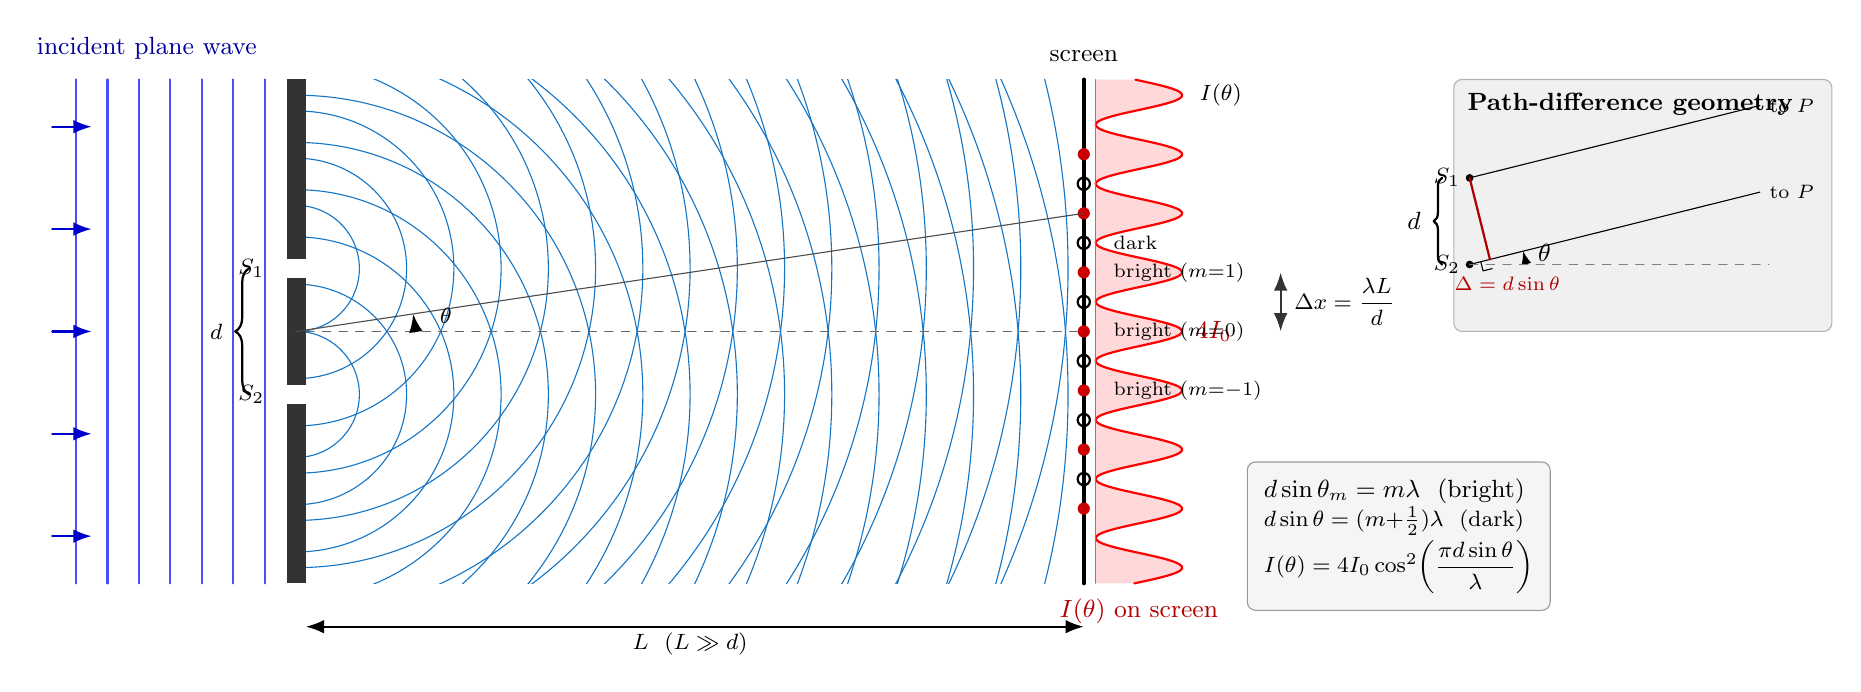
\begin{tikzpicture}[>=Latex,line cap=round,line join=round,font=\footnotesize]

% ---------- Parameters ----------
\def\L{10}              % screen distance
\def\dd{1.6}            % slit separation (exaggerated)
\def\ymax{3.2}          % vertical half-extent
\def\fspacing{0.75}     % fringe spacing on screen
\def\Iamp{1.1}          % amplitude of intensity curve
\def\Ioff{10.15}        % baseline x for intensity curve (= L + 0.15)

% ---------- Incident plane wave (blue parallel lines, left of slits) ----------
\foreach \xi in {-2.8,-2.4,-2.0,-1.6,-1.2,-0.8,-0.4} {
  \draw[blue!70,thick] (\xi,-\ymax) -- (\xi,\ymax);
}
% Arrows indicating propagation direction
\foreach \yi in {-2.6,-1.3,0,1.3,2.6} {
  \draw[->,blue!80!black,thick] (-3.1,\yi) -- (-2.6,\yi);
}
\node[blue!60!black] at (-1.9,{\ymax+0.4}) {\small incident plane wave};

% ---------- Barrier with two slits ----------
\fill[black!80] (-0.12,{\dd/2+0.12}) rectangle (0.12,\ymax);
\fill[black!80] (-0.12,{-\dd/2+0.12}) rectangle (0.12,{\dd/2-0.12});
\fill[black!80] (-0.12,-\ymax) rectangle (0.12,{-\dd/2-0.12});

% Slit labels
\node[left=3pt] at (-0.18,{\dd/2}) {$S_1$};
\node[left=3pt] at (-0.18,{-\dd/2}) {$S_2$};

% Slit separation brace
\draw[decorate,decoration={brace,amplitude=5pt,mirror},thick]
  (-0.6,{\dd/2}) -- (-0.6,{-\dd/2}) node[midway,left=6pt] {$d$};

% ---------- Secondary spherical waves (concentric arcs from each slit) ----------
\begin{scope}
  \clip (0.12,-\ymax) rectangle ({\L-0.05},\ymax);
  \foreach \r in {0.8,1.4,2.0,2.6,3.2,3.8,4.4,5.0,5.6,6.2,6.8,7.4,8.0,8.6,9.2,9.8} {
    \draw[cyan!55!blue,thin] (0,{\dd/2}) circle (\r);
    \draw[cyan!55!blue,thin] (0,{-\dd/2}) circle (\r);
  }
\end{scope}

% ---------- Screen ----------
\draw[black,line width=1.4pt] (\L,-\ymax) -- (\L,\ymax);
\node[above] at (\L,{\ymax+0.1}) {\small screen};

% Distance label L
\draw[<->,thick] (0.12,{-\ymax-0.55}) -- (\L,{-\ymax-0.55});
\node[below] at ({\L/2},{-\ymax-0.5}) {$L$ \ ($L\gg d$)};

% ---------- Intensity curve I(theta) on screen (to the right of screen) ----------
% x of curve = Ioff + Iamp * cos^2(pi * y / fspacing)
\begin{scope}
  \fill[red!15] plot[domain=-\ymax:\ymax,samples=240,smooth]
    ({\Ioff+\Iamp*(cos(180*\x/\fspacing))*(cos(180*\x/\fspacing))},\x)
    -- ({\Ioff},\ymax) -- ({\Ioff},-\ymax) -- cycle;

  \draw[red,thick,smooth,samples=240,domain=-\ymax:\ymax]
    plot ({\Ioff+\Iamp*(cos(180*\x/\fspacing))*(cos(180*\x/\fspacing))},\x);
\end{scope}

% baseline of intensity axis
\draw[black!50,very thin] (\Ioff,-\ymax) -- (\Ioff,\ymax);

% Intensity peak / axis labels
\node[red!70!black,right] at ({\Ioff+\Iamp+0.05},0) {\small $4I_0$};
\node[right] at ({\Ioff+\Iamp+0.1},{\ymax-0.2}) {$I(\theta)$};
\node[red!70!black] at ({\Ioff+\Iamp/2},{-\ymax-0.35}) {\small $I(\theta)$ on screen};

% ---------- Bright/dark markers on screen ----------
% Bright fringes at y = m * fspacing (m = -3..3)
\foreach \m in {-3,-2,-1,0,1,2,3} {
  \pgfmathsetmacro{\yb}{\m*\fspacing}
  \fill[red!80!black] (\L,\yb) circle (2.2pt);
}
% Dark fringes at y = (m+1/2) * fspacing
\foreach \m in {-3,-2,-1,0,1,2} {
  \pgfmathsetmacro{\yd}{(\m+0.5)*\fspacing}
  \draw[black,thick] (\L,\yd) circle (2.2pt);
}
% Fringe-type labels
\node[right=5pt,font=\scriptsize] at ({\L+0.08},0) {bright ($m{=}0$)};
\node[right=5pt,font=\scriptsize] at ({\L+0.08},\fspacing) {bright ($m{=}1$)};
\node[right=5pt,font=\scriptsize] at ({\L+0.08},{1.5*\fspacing}) {dark};
\node[right=5pt,font=\scriptsize] at ({\L+0.08},-\fspacing) {bright ($m{=}{-}1$)};

% ---------- Ray from midpoint of slits to point P on screen (angle theta) ----------
\pgfmathsetmacro{\yP}{1.5}
\coordinate (M) at (0,0);
\coordinate (P) at (\L,\yP);

% optical axis (dashed central horizontal line)
\draw[dashed,black!60] (0.12,0) -- (\L,0);

% ray from slit midpoint to P
\draw[black!70,thin] (M) -- (P);

% angle theta
\pgfmathsetmacro{\thetadeg}{atan2(\yP,\L)}
\draw[->,thick] (1.5,0) arc (0:\thetadeg:1.5);
\node at (1.9,0.2) {$\theta$};

% ---------- Fringe spacing Delta x on screen ----------
\draw[<->,thick,black!80] ({\L+2.5},0) -- ({\L+2.5},\fspacing);
\node[right] at ({\L+2.55},{\fspacing/2}) {$\Delta x=\dfrac{\lambda L}{d}$};

% ---------- Path-difference inset (right side, separate light-gray box) ----------
\begin{scope}[shift={({\L+4.9},1.4)}]
  \pgfmathsetmacro{\insetW}{4.6}
  \pgfmathsetmacro{\insetH}{3.2}
  \fill[black!6,rounded corners=3pt] (-0.2,-1.4) rectangle (\insetW,{\insetH-1.4});
  \draw[black!30,rounded corners=3pt] (-0.2,-1.4) rectangle (\insetW,{\insetH-1.4});

  % Two slit points
  \coordinate (s1) at (0,0.55);
  \coordinate (s2) at (0,-0.55);
  \fill (s1) circle (1.4pt) node[left] {$S_1$};
  \fill (s2) circle (1.4pt) node[left] {$S_2$};
  \draw[decorate,decoration={brace,amplitude=3pt,mirror},thick]
    (-0.35,0.55) -- (-0.35,-0.55) node[midway,left=4pt] {\small $d$};

  % Parallel rays to distant P
  \pgfmathsetmacro{\rl}{3.8}
  \pgfmathsetmacro{\ang}{14}
  \coordinate (e1) at ({\rl*cos(\ang)},{0.55+\rl*sin(\ang)});
  \coordinate (e2) at ({\rl*cos(\ang)},{-0.55+\rl*sin(\ang)});
  \draw[black] (s1) -- (e1);
  \draw[black] (s2) -- (e2);
  \node[right,font=\scriptsize] at (e1) {to $P$};
  \node[right,font=\scriptsize] at (e2) {to $P$};

  % Foot of perpendicular from S1 onto line through S2 (parallel to e2 direction)
  \pgfmathsetmacro{\vx}{cos(\ang)}
  \pgfmathsetmacro{\vy}{sin(\ang)}
  \pgfmathsetmacro{\proj}{1.1*\vy}
  \coordinate (F) at ({\proj*\vx},{-0.55+\proj*\vy});

  % Draw perpendicular short line from S1 to F (this is the path-difference segment)
  \draw[red!70!black,thick] (s1) -- (F);

  % small right-angle marker at F
  \pgfmathsetmacro{\sx}{0.12*\vx}
  \pgfmathsetmacro{\sy}{0.12*\vy}
  \pgfmathsetmacro{\pxx}{-0.12*\vy}
  \pgfmathsetmacro{\pyy}{0.12*\vx}
  \draw[black,thin]
    ($(F)+(-\sx,-\sy)$) -- ($(F)+(-\sx-\pxx,-\sy-\pyy)$)
    -- ($(F)+(-\pxx,-\pyy)$);

  % Angle theta at S2 (between dashed horizontal and ray to P)
  \draw[->,thin] ($(s2)+(0.7,0)$) arc (0:\ang:0.7);
  \node at ($(s2)+(0.95,0.15)$) {\small $\theta$};

  % Dashed horizontal reference through S2
  \draw[dashed,black!50] (s2) -- ($(s2)+(\rl,0)$);

  % Label Delta = d sin theta
  \node[red!70!black,font=\scriptsize]
    at ({0.5*\proj*\vx+0.35},{-0.55+0.5*\proj*\vy-0.28})
    {$\Delta=d\sin\theta$};

  % Inset title
  \node[anchor=north west] at (-0.15,{\insetH-1.45})
    {\small \textbf{Path-difference geometry}};
\end{scope}

% ---------- Formula box (bottom right) ----------
\node[draw=black!40,fill=black!4,rounded corners=3pt,inner sep=6pt,align=left]
  at ({\L+4.0},-2.6)
  {\small $d\sin\theta_m=m\lambda$ \ (bright)\\[1pt]
          $d\sin\theta=(m{+}\tfrac{1}{2})\lambda$ \ (dark)\\[1pt]
          $I(\theta)=4I_0\cos^{2}\!\left(\dfrac{\pi d\sin\theta}{\lambda}\right)$};

\end{tikzpicture}
\end{document}
